\documentclass[xcolor=table,final,hyperref={pdfpagelabels=false}]{beamer}
% February 9, 2016
% http://tex.stackexchange.com/a/38609/17923
\usepackage{etex}

\usepackage{grffile}
\usepackage{minted}
\usepackage{wrapfig}
\mode<presentation>{\usetheme{UCTCSOE16}} %%%UCTCSOE16, FutureSOC, HPIUCT, CSUCT, Neat, Aachen, I6dv, I6pd2, I6pd, I6td
\usepackage[utf8]{inputenc}
\usepackage[english, russian]{babel}
\usepackage[T1]{fontenc}
\usepackage{amsmath,amsthm, amssymb, latexsym}
%\usepackage{times}\usefonttheme{professionalfonts}  % obsolete
%\usefonttheme[onlymath]{serif}
\boldmath
\usepackage[orientation=portrait,size=a1,scale=1.4,debug]{beamerposter}
% change list indention level
% \setdefaultleftmargin{3em}{}{}{}{}{}


%\usepackage{snapshot} % will write a .dep file with all dependencies, allows for easy bundling

\usepackage{array,booktabs,tabularx}
\newcolumntype{Z}{>{\centering\arraybackslash}X} % centered tabularx columns
\newcommand{\pphantom}{\textcolor{ta3aluminium}} % phantom introduces a vertical space in p formatted table columns??!!

%%%\usepackage{authblk}

\usepackage{tikz}
\usepackage{xcolor}
\usepackage{multirow}

\usepackage{comment}
\usepackage{verbatim}
\usepackage[skip=0pt]{caption}

% February 8, 2016
% http://tex.stackexchange.com/a/91580/17923
\usepackage[export]{adjustbox}

\usepackage{enumerate}

% November 21, 2016
% http://tex.stackexchange.com/a/144342/17923
\usepackage[many]{tcolorbox}

\usepackage{ragged2e}
\justifying

% November 21, 2016
% http://tex.stackexchange.com/a/32822/17923
% \newcommand{\UCTCSOEposterhighlight}[2][l]{%
%   \colorbox{infocolorgray}{\begin{tabular}{@{}#1@{}}#2\end{tabular}}%
% }


\listfiles

%%%%%%%%%%%%%%%%%%%%%%%%%%%%%%%%%%%%%%%%%%%%%%%%%%%%%%%%%%%%%%%%%%%%%%%%%%%%%%%%%%%%%%
\graphicspath{{figures/}}
 
\title{Использование методов, основанных на кросс-энтропии, для снижения размерности временных рядов}
\author{Использование методов, основанных на кросс-энтропии, для снижения размерности временных рядов}
\institute{Махнева Лиза}

\date[2019]{2019}

\hypersetup{linkcolor=blue,citecolor=blue,urlcolor=blue,bookmarks=true,bookmarksnumbered=true}

\hypersetup{
   pdfinfo={
      Title={Streamlining Technology-driven Orchestration in Formal Learning Spaces}, 
      Author={Lighton Phiri}, 
      Subject={Technology Enhanced Learning}, 
      Keywords={Educational Technology, Orchestration, TEL, Technology Enhanced Learning},
      CreationDate={D:20161119234910}%%%,
      %%%ModDate={D:20150330150057}
   }
}
%%%%%%%%%%%%%%%%%%%%%%%%%%%%%%%%%%%%%%%%%%%%%%%%%%%%%%%%%%%%%%%%%%%%%%%%%%%%%%%%%%%%%%
\newlength{\columnheight}
\setlength{\columnheight}{105cm}

\newcommand\ytl[2]{
\parbox[b]{8em}{\hfill{\color{black}\bfseries\sffamily #1}~$\cdots\cdots$~}\makebox[0pt][c]{$\bullet$}\vrule\quad \parbox[c]{4.5cm}{\vspace{7pt}\color{black!80}\raggedright\sffamily #2.\\[7pt]}\\[-3pt]}

\begin{document}
\begin{frame}
  
  \vspace{1cm}
  
  \begin{columns}[t, totalwidth=0.98\textwidth]
    % ---------------------------------------------------------%
    % Set up a column 
    \begin{column}{.51\textwidth}
      \begin{beamercolorbox}[center,wd=\textwidth]{postercolumn}
        \begin{minipage}[T]{.95\textwidth}  % tweaks the width, makes a new \textwidth
          \parbox[t][\columnheight]{\textwidth}{ % must be some better way to set the the height, width and textwidth simultaneously
            % Since all columns are the same length, it is all nice and tidy.  You have to get the height empirically
            % ---------------------------------------------------------%
            % fill each column with content   
            \vskip-1ex

            \begin{block}{Энтропия $H(X)$}
               \vskip-1ex
              
% % % % %                 \colorbox{infocolorgray}{\strut \textcolor{ta2orange}{\; Workflow scenario involves four core steps\\ involving pre-session management (Steps 1--3) and session management (Step 4). \;}}
% % % % %                 \vskip 1ex
                
                \justifying В случае дискретных случайных величин энтропия показывает минимальное среднее число бит для шифрования информации о значениях, которые принимает случайная величина.
            \begin{equation*}
	            H(X) = \sum_{i=1}^{n}p_i \cdot \log_2 {\frac{1}{p_i}} = -\sum_{i=1}^{n}p_i \cdot \log_2 p_i \, ,
            \end{equation*}
                \justifying где $p_i$ --- вероятность того, что случайная величина $X$ примет i-ое значение.
            \end{block}
            \vskip-1.5ex
            \begin{block}{Кросс-энтропия}
                \vskip-1ex
                 \justifying Это количество информации, в среднем, необходимое для опознания событий из распределения $P$, используя оптимальную схему для распределения $\tilde P$.
                \begin{equation*}
	                H_P(\tilde P) = -\sum_{i=1}^{n} p_i \cdot \log_2 \tilde{p_i}
                \end{equation*}
		    \end{block}
		    \vskip-2ex
		    \begin{block}{Дивергенция Кульбака-Лейблера}
		    \vskip-1ex
		        \justifying Данная величина является разностью кросс-энтропии и энтропии. С ее помощью можно определить, какое количество информации мы потратили сверх необходимого из-за того, что не знаем истинное распределение случайной величины. Поэтому она показывает степень отдаленности одного вероятностного распределения $P$ от другого $\tilde P$.
		        \begin{equation*}
	                D_{KL}(P\, ||\, \tilde P) = - \sum\limits_{i=1}^n p_i\log \tilde p_i + \sum\limits_{i=1}^n p_i\log p_i
                \end{equation*}
		    \end{block}
		    \vskip-1.5ex
		    \begin{block}{Применение кросс-энтропии}
		        \vskip-1ex
		        \justifying В алгоритме UMAP используется дивергенция Кульбака-Лейблера для случайной величины Бернулли $X \sim B(p(x))$:
                \begin{equation*}
	                p(x)\log \frac{p(x)}{\tilde p(x)} + (1 - p(x))\log \frac{1 - p(x)}{1 - \tilde p(x)}
                \end{equation*}

                \justifying Однако алгоритм рассчитывает сумму таких разниц для $n$ случайных величин (для 2 множеств из $n$ случайных величин, $S$ и $\tilde S$):
                \begin{equation*}
	                \sum_{i=1}^n \left(p(x_i)\log \frac{p(x_i)}{\tilde p(x_i)} + (1 - p(x_i))\log \frac{1 - p(x_i)}{1 - \tilde p(x_i)}\right)
                \end{equation*}

                \justifying Минимизация $C_S(\tilde S)$ по $\tilde p(x)$ позволяет найти множество $\tilde S$, которое наиболее похоже на множество $S$.

		    \end{block}
		    \vskip2.5ex
		    \noindent\rule{\textwidth}{1pt}
		    \vskip0.5ex
		    \begin{block}{Реализация UMAP}
		        \vskip-1ex
		        \justifying Применим алгоритм к данным о ценах криптовалют на протяжении 669 дней (см. рис \ref{pic}). Рассмотрим сформировавшийся кластер №1. Временные ряды, оказавшиеся в кластере, ведут себя наиболее похоже во времени. Они сильно коррелируют между собой:
		        \begin{figure}
		        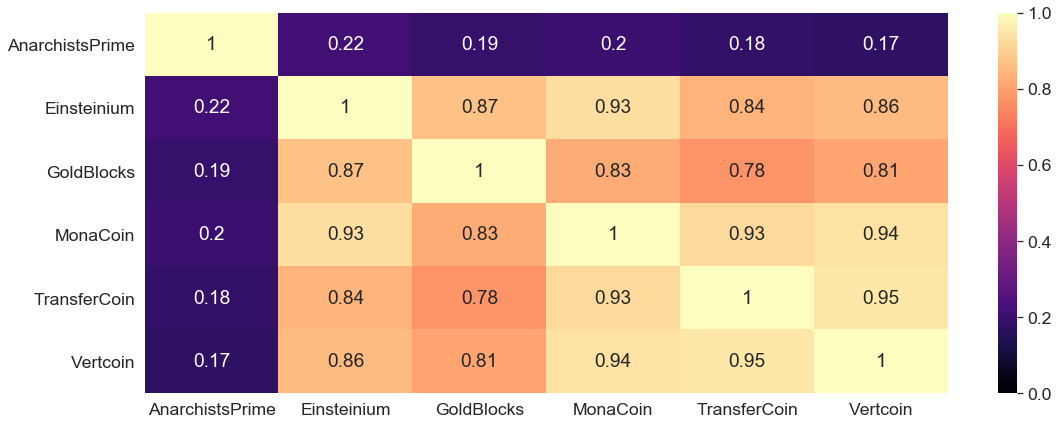
\includegraphics[width=\linewidth]{charts/corr}
		        \caption{Коэффициенты корреляции между рядами кластера №1}
		        \label{2}
		        \end{figure}
		        \vskip-1.5ex
		        \justifying Однако AnarchistsPrime выбивается из группы криптовалют --- у нее самые низкие коэффициенты корреляции. Если посчитать корреляцию AnarchistsPrime со всеми временными рядами из выборки, получается, что наибольшее значение равно $0.22$. То есть криптовалюта оказалась в данном кластере, так как в нем наиболее близкие к ней объекты среди имеющихся.\\[4mm]
		        \justifying Значит, UMAP и коэффициент корреляции по-разному оценивают схожесть рядов. Алгоритм считает похожими те, между которыми оказалось наименьшее «расстояние», даже если это расстояние велико — просто в представленной выборке не оказалось объектов ближе.
		        
		    \end{block}
            \vskip-1ex
          }
        \end{minipage}
        
      \end{beamercolorbox}
    \end{column}
    % ---------------------------------------------------------%
    % end the column

    % ---------------------------------------------------------%
    % Set up a column 
    \begin{column}{.47\textwidth}
      \begin{beamercolorbox}[center,wd=\textwidth]{postercolumn}
        \begin{minipage}[T]{.95\textwidth} % tweaks the width, makes a new \textwidth
          \parbox[t][\columnheight]{\textwidth}{ % must be some better way to set the the height, width and textwidth simultaneously
            % Since all columns are the same length, it is all nice and tidy.  You have to get the height empirically
            % ---------------------------------------------------------%
            % fill each column with content
            \vskip-1ex
              %%%%%\vskip-2ex
              %%%%%\begin{block}{1) Orchestrating a Flipped Class}
		    \begin{block}{Алгоритм UMAP (Uniform Manifold Approximation and Projection)}
		    \begin{center}
		    \vskip-4ex
		    \begin{tabular}{|c|p{0.5cm}|p{0.5cm}|p{0.5cm}|p{0.5cm}|p{0.5cm}|p{0.5cm}|p{7cm}|c|p{0.5cm}|p{0.5cm}|p{0.5cm}|p{0.5cm}|}
	        \cline{1-7}
	        \cline{9-13}
	        & \multicolumn{6}{c|}{$D$ признаков} & \multirow{5}{6cm}{$\qquad \; \; \longrightarrow$} & \multicolumn{5}{c|}{$d$ признаков}\\
	        \cline{1-7}
	        \cline{9-13}
	        \multirow{4}{*}{$k$ объектов} & & & & & & & & \multirow{4}{*}{$k$ объектов} & & & &\\
	        \cline{2-7}
	        \cline{10-13}
	        & & & & & & & & & & & &\\
	        \cline{2-7}
	        \cline{10-13}
	        & & & & & & & & & & & &\\
	        \cline{2-7}
	        \cline{10-13}
	        & & & & & & & $ \qquad D \gg d$ & & & & &\\
	        \cline{1-7}
	        \cline{9-13}
          \end{tabular}
		  \end{center}
	      
	      \vskip2ex
	      
            
		  \begin{center}
		      \bfseries{\large{Принцип работы
		      алгоритма}}
		  \end{center}
		  \vskip1ex
	      \begin{minipage}[t]{\textwidth}
		  \tcboxfit[width=25.5cm,height=15.8cm,title={\large Построение графа}, colback=white, colframe=mine,  borderline={0pt}{0pt}{black}]{
		  \begin{itemize}
		     \justifying 
		     \normalsize
		     \leftskip -0.3in
		     \normalitem Для каждого объекта из выборки UMAP находит $k$ ближайших соседей, рассчитывает расстояние $\rho$ до ближайшего, а также нормирующую величину $\sigma$
		     \normalitem Затем UMAP строит ориентированный взвешенный граф: ребрами соединяются каждый объект с его соседями. Вес ребра из объекта $x_i$ к его соседу $t_j$ определяется по формуле:
		     \begin{equation*}
	            w(x_i \rightarrow t_j) = \exp\left(-\frac{d(x_i, t_j) - \rho_i}{\sigma_i}\right)
            \end{equation*}
            \normalitem Если интерпретировать вес ребра из $a$ в $b$ как вероятность его существования, то мы можем определить вес ребра между $a$ и $b$ как вероятность существования хотя бы одного ребра:
            \begin{equation*}
	            w(a,b) = w(a \rightarrow b) + w(b \rightarrow a) - w(a \rightarrow b) \cdot w(b \rightarrow a)
            \end{equation*}
		     %%%%%\normalitem Associate resources to activities.
		  \end{itemize}}
		  
	      \end{minipage}%
	      \vspace{0.5cm}
	      \begin{minipage}[t]{\textwidth}
	      
		\tcboxfit[width=25.5cm,height=14.2cm,title={\large Снижение размерности}, colback=white, colframe=my,  borderline={0pt}{0pt}{black}]{
		    \begin{itemize}
		    \justifying
		    \normalsize
		     \leftskip -0.3in
		     \normalitem Ребро $e$ является случайной величиной: $e \sim B(w(e))$. Множество ребер построенного графа --- множество $E$ из случайных величин Бернулли
		     \normalitem Чтобы перенести граф в низкоразмерное пространство, UMAP подбирает для множества~$E_h$ похожее на него множество~$E_l$ с функцией~$w_l(e)$, соответствующие низкоразмерному пространству
		     \normalitem UMAP решает задачу минимизации кросс-энтропии:
            \begin{equation*}
	            -\sum_{e \in E} w_h(e)\log w_l(e) + (1 - w_h(e))\log (1 - w_l(e)) \rightarrow \min_{w_l}
            \end{equation*}
            Результатом является граф в низкоразмерном пространстве с подобранной функцией весов $w_l$.
		    \end{itemize}

		  }
		  \vskip1.35ex
		  \noindent\rule{\textwidth}{1pt}
		  \vskip9ex
		  \begin{center}
		  \begin{figure}
          \noindent \centering 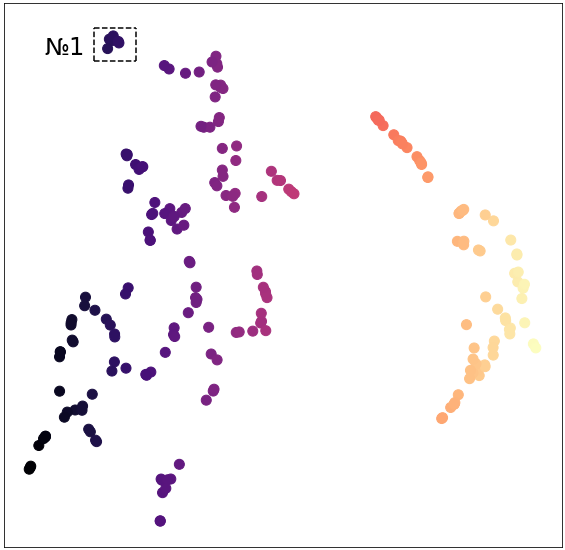
\includegraphics[width=0.9\linewidth]{charts/show}
          \caption{Результат работы UMAP с временными рядами криптовалют}
          \label{pic}
          \end{figure}
		  \end{center}
	      \end{minipage}%
	      \end{block}
          }
          
          % tcboxfit
        \end{minipage}
      \end{beamercolorbox}
    \end{column}
  \end{columns}
\end{frame}
\end{document}


%%%%%%%%%%%%%%%%%%%%%%%%%%%%%%%%%%%%%%%%%%%%%%%%%%%%%%%%%%%%%%%%%%%%%%%%%%%%%%%%%%%%%%%%%%%%%%%%%%%%
%%% Local Variables: 
%%% mode: latex
%%% TeX-PDF-mode: t
%%% End:
